\documentclass[12pt,a4paper,twoside]{report}
\usepackage[utf8]{inputenc}
\usepackage[english]{babel}
\usepackage{indentfirst}
% \usepackage{enumitem}
\usepackage{pdfpages}


\usepackage{listings}
\usepackage{color}

\usepackage{graphicx}
\graphicspath{ {./images/} }

\usepackage{cite}
\usepackage{hyperref}
\hypersetup{
	colorlinks=false,
	linkcolor=blue,
	filecolor=magenta,
	urlcolor=cyan,
}

\title{Master thesis}
\author{Tomáš Belluš}

\definecolor{codegreen}{rgb}{0,0.6,0}
\definecolor{codegray}{rgb}{0.5,0.5,0.5}
\definecolor{codepurple}{rgb}{0.58,0,0.82}
\definecolor{backcolor}{rgb}{0.95,0.95,0.95}

\lstdefinestyle{codestyle}{
	commentstyle=\color{blue},
	keywordstyle=\color{black},
	numberstyle=\tiny\color{codegray},
	stringstyle=\color{codepurple},
	showstringspaces=false,
	captionpos=b,
}
\lstset{style=codestyle}

\lstdefinestyle{appendix}{
	basicstyle=\small\ttfamily,
	showstringspaces=false,
	captionpos=b,
	numbers=left,
	stepnumber=1,
	numberstyle=\small,
	breaklines=true,
}

\usepackage[utf8]{inputenc}
\usepackage[T1]{fontenc}
\usepackage[english]{babel}
\usepackage[a4paper]{geometry}
\usepackage[
    left = \glqq,% 
    right = \grqq,% 
    leftsub = \glq,% 
    rightsub = \grq%
]{dirtytalk}

% SETTINGS - NAMES
\newcommand{\myTitle}[0] {Bait network based monitoring of malicious actors}
\newcommand{\myName}[0] {Tomáš Belluš}
\newcommand{\mySupervisor}[0] {Ing. Tibor Csóka, PhD.}
\newcommand{\myEvidenceNumber}[0] {FIIT-XXXXXX-82385}
\newcommand{\myDate}[0] {May 2020}
\newcommand{\myStudyProgram}[0] {Information Security}
\newcommand{\myStudyField}[0] {9.2.4 Computer Engineering}
\newcommand{\myInstitude}[0] {Institute of Computer Engineering and Applied Informatics}

\usepackage[parfill]{parskip}
\usepackage{enumitem}

\usepackage{graphicx}
\usepackage{float}
\usepackage{longtable}
\usepackage{setspace}

% Spacing
\setstretch{\mySpacing}

\setcounter{secnumdepth}{3}
\setcounter{tocdepth}{3}

\usepackage{tabularx}
\newsavebox\mybox
\usepackage{fancyhdr}
\pagestyle{fancy}
\lhead{\nouppercase{\leftmark}}
\chead{}
\rhead{}
\lfoot{}
\cfoot{\thepage}
\rfoot{}


%style=iso-numeric
%style=authortitle-dw
\usepackage[maxnames=1,backend=bibtex,defernums=true]{biblatex}
\defbibheading{references}[Literature]{ 
  \chapter*{#1}
  \markboth{#1}{#1}
}
%\defbibheading{referencessec}[Literature]{ 
%  \section*{#1}
%  \markboth{#1}{#1}
%}
\bibliography{\myBibliography}


% Listing as figure
%\usepackage{libs/minted}
%\usepackage[section]{minted}

\usepackage{listing}

% openright does not work :(
\let\tmp\oddsidemargin
\let\oddsidemargin\evensidemargin
\let\evensidemargin\tmp
\reversemarginpar

\usepackage{lscape}
\usepackage{afterpage}

\usepackage{lipsum}
\usepackage{hyperref}

\begin{document}
	
%title page
\begin{center}
\thispagestyle{empty}
{\Large Slovak University of Technology in Bratislava}
\par\end{center}{\Large \par}

\begin{center}
{\Large Faculty of Informatics and Information Technologies}
\par\end{center}{\Large \par}

\smallskip{}

\begin{center}
\myEvidenceNumber
\par\end{center}
\vfill{}

\begin{center}
\textbf{\Large \myName}
\par\end{center}{\Large \par}

\medskip{}


\begin{center}
\textbf{\LARGE \myTitle }
\par\end{center}{\huge \par}

\medskip{}


\begin{center}

{\Large Výskumný zámer}
\par\end{center}{\Large \par}

\vfill{}

\noindent
Study program: \myStudyProgram

\noindent
Field of study: \myStudyField

\noindent
Training workplace: \myInstitude

\noindent
Supervisor: \mySupervisor

\medskip{}

\noindent
\myDate


\newpage
\thispagestyle{empty}
\mbox{}
\newpage



%assignment
%\thispagestyle{empty}

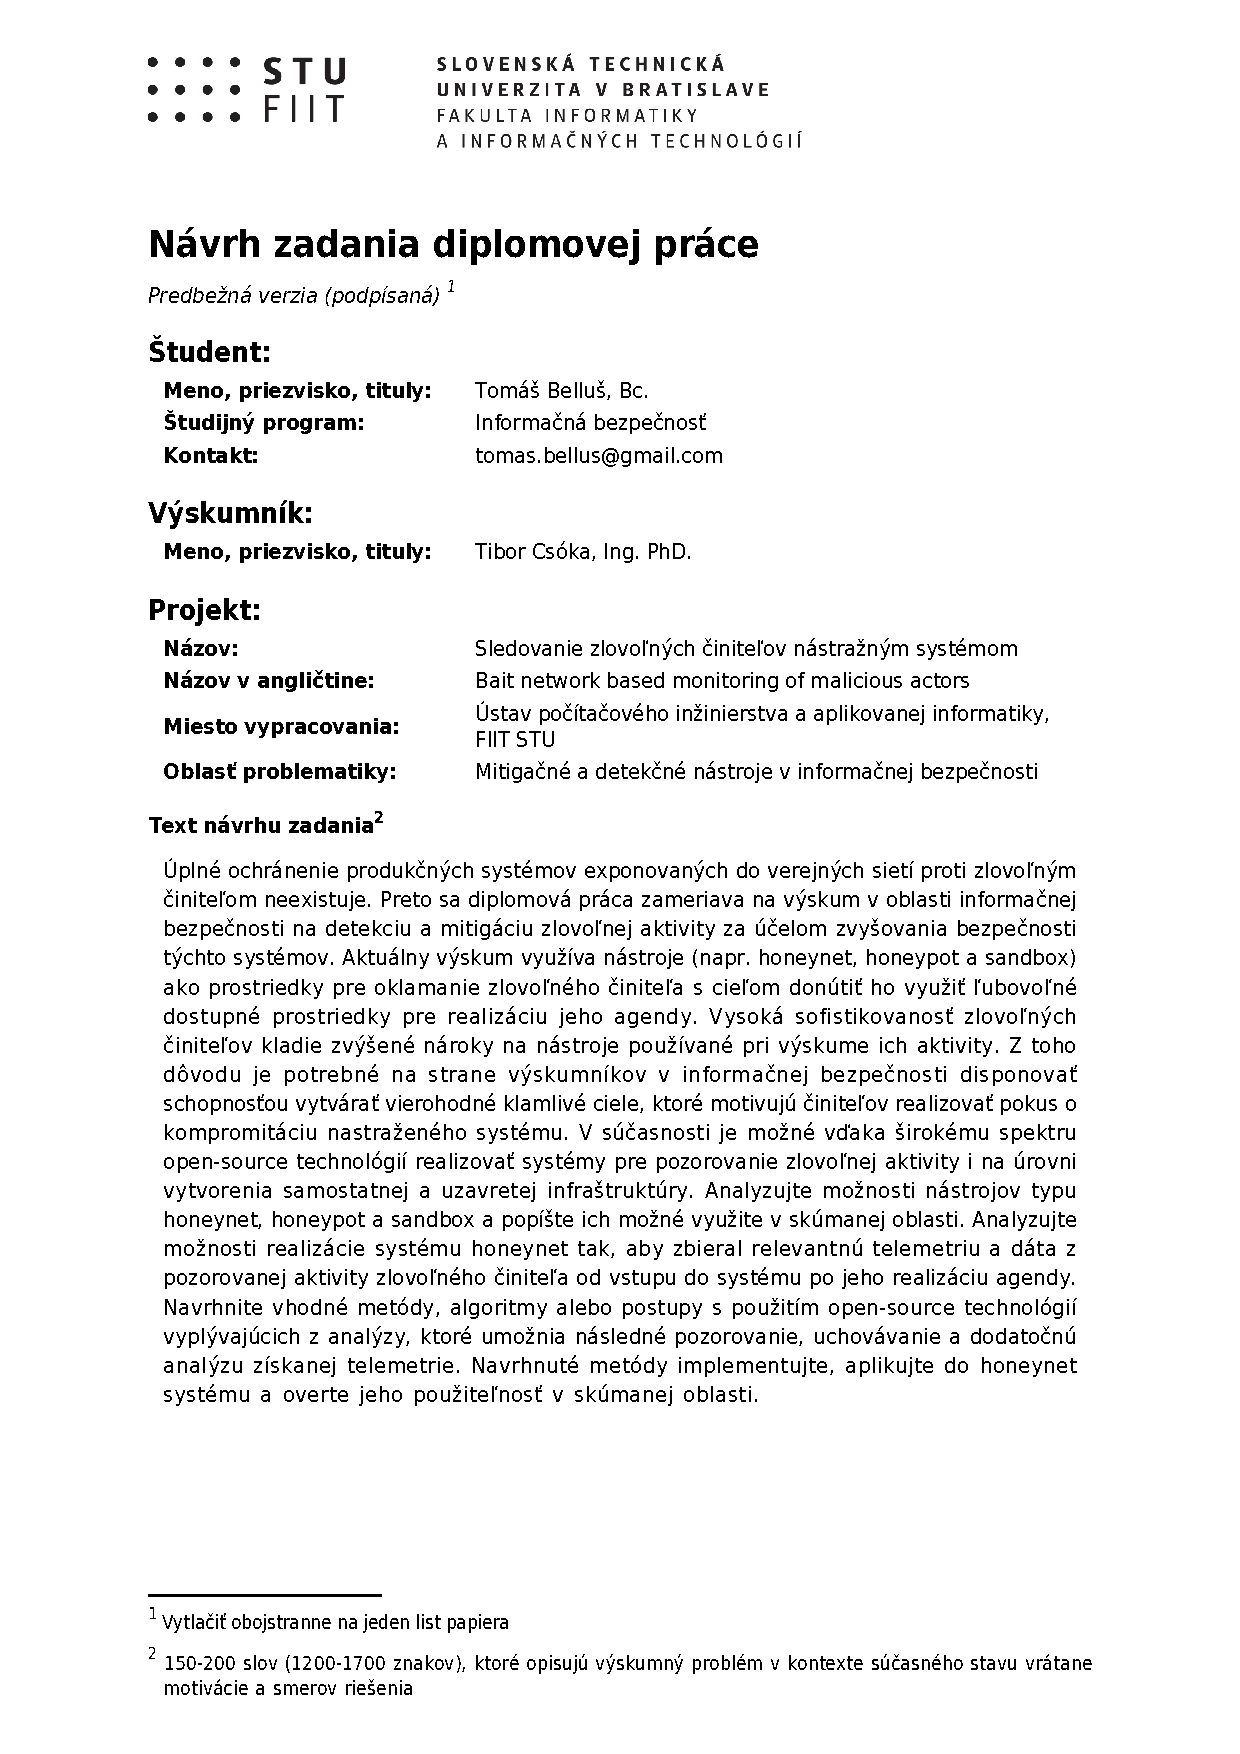
\includepdf[pages=-]{preamble/dp_zadanie.pdf}

%\newpage{}
%\thispagestyle{empty}

%\newpage
%\thispagestyle{empty}
%\mbox{}
%\newpage

% table of contents
\begingroup
\color{black}
\tableofcontents
\endgroup


\chapter{Motivation}\label{motivation}

Threat intelligence research often focuses on solving a variety of questions important for better understanding the paradigms and techniques used in securing these systems, some of the more common are:
\begin{enumerate}
	\item How can systems be exploited?
	\item How does a malicious actor obtain foothold inside the system?
	\item What techniques could the malicious actor use?
\end{enumerate}

There is a variety of approaches to identifying practices and techniques used by the malicious actors, e.g. post-mortem incident analysis \cite{research:blog:post-mortem} or proactive malicious actor baiting using honeypots and honeynets \footnote{Honyenet is a robust network honeypot consisting network components used to detect network vulnerabilities \cite{research:web:honeynet}.}.

%- ked preventivne zistime, ake 0day existuju, alebo ake postupy pouzivaju automatizovane utociace systemy, nestoji nas to nic... lebo ziaden incident sa nestal, informacie ziskane z honeypotov a honeysieti je potom mozne disseminate do praxe
%  - obmedzenie - ked sa niekto zamera... na nieco, ako napr. targeted utok na debila na PR oddeleni, ktori dostane phishing,... v honeypote/honeynete ho neuvidime... ;)
%- incident - nieco sa posralo a kapitalne sa dokakalo, systemy boli narusene... to je pekne, ze nieco mozno z incidentu vytiahneme... ale sikovny utocnik... vie po sebe aj pekne pozametat... a nemusime sa k niecomu byt schopni dostat... ;)

 
Malicious actors follow a multi-phase process \cite{research:seven-phases} \cite{research:seven-phases2} to completely plan the sophisticated attack. The phases fall under so called Cyber/Intrusion Kill Chain and include - reconnaissance, weaponization, delivery, exploitation, installation, command and control, actions on objective. Briefly, the attack begins with analyzing and discovering the target objective, followed by preparation of the exploit to compromise the system and getting required control to fulfill a goal. The idea is related to the US military process of targeting (F2T2EA), where any failure breaks the chain \cite{research:paper:kill-chain}. 

As well as the malicious actors, security experts can use equally complex tools and practices to detect, mitigate or reproduce an attack.
Tools like sandboxes, sinkholes, honeypots and many active detection tools (e.g.~WAF, IPS/IDS, FW, etc.). 

Typical practice among security experts is to study the hacking practices by practicing ethical hacking often abbreviated as a "red" team. While the opposing team is known as the "blue" team - mitigating, detecting and stopping the activity. In the "fight" of blue versus red, the blue team must keep up with the red teams' new state-of-the-art techniques and zero-day exploitations. Zero-day exploitation targets vulnerabilities not yet addressed by vendors and not publicly disclosed
\cite{research:symantec:zero-day}. Such vulnerabilities are almost impossible to mitigate and very difficult to detect. White hat or ethical hackers - hackers looking for exploits with no intent to harm - search for these vulnerabilities in their own environments by reading all those lines of code or dynamically - utilizing honeypots.
% collecion of intelligence from the attacked by baiting them to release their techniques/tools on useless infra

Crucial element of a honeypot is the ability to quickly reconfigure or duplicate it into a new environment. Regarding that honeypots are vulnerable to zero-day vulnerabilities, it must be mitigated either by catching th maliscious actor on the peripheral systems (via Firewall ACLs) or by the ability to recover from the breakdown by restoring the honeypot's state.
% the lowest cost is associated with detecting 0day vulnerabilities on infrastructure dedicated to catching the malicious actor on the peripheral systems.

\chapter{Analysis}\label{analysis}

% virtualization - protective layer
"The primary technology that makes immutable infrastructure possible at any scale is virtualization (both software and hardware) across networking, servers, and storage" \cite{research:sumologic:immutable-infra}. According to this, virtualization is the inseparable element of immutable infrastructure. In terms of security, it operates an isolation layer protecting the underlying layers.

\section{Best practice in infrastructure orchestration}\label{immutable-infrastructure-and-its-orchestration}
\subsection{Evolution}
The evolution of virtualization and rise of containers to even more isolated services (i.e. concepts Software-as-a-Service and Function-as-a-Service) led to resource sharing and its maximum utilization. Application and services are divided compared to the traditional monolithic architectures with all services stacked in one server \cite{research:microservices}.

\subsection{Immutable and idempotent infrastructure}

To understand the applications of immutable infrastructure one must identify its characteristics. Any system or unit of a system (i.e. container, VM, server) is pre-configured and deployed to its final state in a target environment. The state is immutable - it forbids any further configuration changes or additional networking. Required changes are applied in the \emph{infrastructure configuration} (e.g. container images) and redeployed to apply the updated state. In comparison, a mutable infrastructure is the exact opposite, such as almost every computer, that requires manual step-by-step installation of the OS and the underlying applications and network configurations.

"In mathematics, a number that is idempotent keeps the same value when multiplied by itself, no matter how many times the function is applied" \cite{research:idempotence:math}. In computing, it is an operation executed only when the result will differ \cite{research:idempotence:it}. Having a complex infrastructure composed of multiple services allows segmentation. Instead of upgrading/modifying a whole infrastructure, only the desired segments are addressed - idempotent infrastructure \cite{research:ansible-idempotence}. It resides with orchestration and the security of segmentation of services (refer to \autoref{escape-attack-mitigation}). Orchestration is the question of how, when and what combined in a single process of the mechanism used.

The immutability has a profound effect on the security of the infrastructure \cite{research:blog:immutablity-pros}. Since every change is made by redeploying the infrastructure, all footprints of the malicious actor vanish despite possibly being capable of outlasting a reboot.

The immutable infrastructure paradigm ensures the whole environment may be recovered. Usage of immutable infrastructure may introduce the possibility of designing a complex honeynet composed of multiple interconnected network segments and devices. As the whole infrastructure is described in a configuration, the modification of a service is the matter of changing or setting a variable. When such configurations, utilizing the immutability, is used in production, the deployment of mirror infrastructure is matter of configuring the right hosts.
% opytat sa, ci sa da menit nazov temy... ak ano, zvazit vymenu "immutable" za nieco ine -> preco - lebo cela immutable infra ma iba deklarativnu formu immutable = fully automatic

% separation of data and logic - creating as stateless services as possible

\subsubsection{Escape attack mitigation}\label{escape-attack-mitigation}
Escape attacks exploit vulnerabilities in shared resources or stack layer (i.e. kernel for KVM, application for functions or hardware for virtualization). A case study, with a goal to mitigate any form of escape attacks, at the Swedish Police Authority by Christian Abdelmassih - \emph{Docker and Kubernetes in high security environments}. The author discusses application isolation techniques while providing orchestration with Kubernetes.

% tak ako prislo KVM - evolucia - preco by sme nemohli pouzivat ten isty kernel... ale museli per VM vytvarat aj separe kernel... -> bezpecnejsie
One technique is to isolate applications by containerization (e.g.~Docker, LXC, etc.), which share the host's kernel. Second technique is separation by (bare-metal) hypervisor - virtual machines (VM). This means that the VM has it's own operation system (OS) and shares hardware resources of the host. In conclusion, the idea is to
utilize bare-metal hypervisor (cloud native) to minimize the attack surface for escape attacks, because containers are vulnerable to kernel driven escape attacks.

% KVM - OS + KVM - para-virtualization
% Xen - bare metal virtualization

To separate non-related application and utilize containers, he suggests segmentation of Kubernetes pods to logical classes (e.i. class O, class P and class PG) \cite{research:thesis:docker-k8s-security}. These classes are to be organized and orchestrated by Kubernetes and should make sure nodes and pods have the same class tags. Even though the presented solution lacks verification, it introduces well defined concepts, possible applicable for my thesis, as the the author finalizes that "In order to utilize this in clouds in a scalable manner, there are additional requirements for automation that must be satisfied. For example, automating the creation of virtual machines, attaching them to the Kubernetes cluster. Most importantly one must also implement and verify that the application classifications are respected at all times" \cite{research:blog:docker-k8s-security}.

\subsection{Honeypots \& Sandboxes}\label{honeypots-sandboxes}

Both honeypots and sandboxes are similarly used in dynamic threat analysis. Difference is in preparation and isolation. Honeypot monitors the activity of a malicious actor or malware in an emulated or production-like environment. Sandbox is an isolated environment for dynamic malware analysis with all preparation that is needed based on the knowledge of the malware. Usually, honeypots are configured to detect specific attacks with emulated applications or not emulated to detect zero-day vulnerabilities and monitor behavior of potential exploitations \cite{research:enisa:honeypots}. Within a sandbox, all activity is monitored as much as possible, while knowing the outcome of the attack, to know the source of the attack.

% https://www.sciencedaily.com/releases/2017/11/171129164003.htm
% idea older, but can be implemented using fully open-source technology? 

A particularly interesting topic is to \emph{detect zero-day vulnerabilities} in a honeypot and, if necessary, replicating and more in depth analyzing the exploitation in a sandbox. Analyzing malware in a sandbox provides virtualization, which mitigates MBR overwrite. On the other hand, most malwares verify the environment they're in - detection of virtualization or sandbox awareness.

\chapter{Master's thesis overview}\label{masters-thesis-overview}

\section{Research questions}\label{research-questions}

How to improve virtualization/emulation detection in a honeynet/sandbox?

What is the most detectable phase in the Cyber Kill Chain?

The underlying technology for virtualization and containerization (if any) is crucial to reach immutability. What provisioning and orchestration mechanisms are needed to ensure an immutable infrastructure?

What is the best practice of implementing a system for observing a malicious actor?

How to design a deception mechanism baiting the malicious actor to believe in production-like attribution of the system.

\subsection{Thesis goal}\label{thesis-goal}

Design a honeynet, in Linux, as a dynamic analytic tool dedicated to observing the activity of a malicious actor. Utilize the state-of-the-art infrastructure deployment and orchestration paradigms to ensure automated and a secure system. Mitigating escape attacks will not be in scope of this thesis, but the introduced segmentation technique will be taken into account to segregate related services.

\subsection{Plan of work}\label{plan-of-work}

\subsubsection{DP I}\label{dp-i}

\begin{itemize}
\item
  analyze virtualization (e.g KVM), emulation and virtualization detection mitigation practices
\item
  analyze cross-platform orchestration and provisioning mechanisms
\item
  comparison of existing solutions and discussion of possible improvements
\item
  design of the whole stack of the system supported by analysis
\end{itemize}

\subsubsection{DP II}\label{dp-ii}

\begin{itemize}
\item
  discuss observable attack vectors
\item
  implementation of the system skeleton and configuration of the orchestartion mechanism

  \begin{itemize}
  \item
    create base images for the system
  \item
    automated deployment
  \end{itemize}
\item
  document the implementation
\item
  assignment revision if necessary
\end{itemize}

\subsubsection{DP III}\label{dp-iii}

\begin{itemize}
\item
  test honeynet implementation on live server
\item
  analyze all retrieved data and indicators of compromise
\item
  apply required modifications to images or core functionality
\item
  finalize the thesis documentation and evaluate reached goals
\end{itemize}

\chapter{Further Literature}\label{further-literature}

\begin{enumerate}
	\item paper on \emph{Zero-Day Attack Signatures Detection Using Honeypot} \url{https://pdfs.semanticscholar.org/d4e4/5e81b8d8878ca99648c3fc890ede1ae01b49.pdf}
	
	\item thesis on \emph{Docker and Kubernetes in high security environments} \url{https://kth.diva-portal.org/smash/get/diva2:1231856/FULLTEXT02.pdf}
	
	\item paper on \emph{Adaptive and Flexible Virtual Honeynet}
	\url{https://www.researchgate.net/publication/285598988_Adaptive_and_Flexible_Virtual_Honeynet}
	
	\item conference paper on \emph{Automated Configuration of Monitoring Systems in an Immutable Infrastructure} \url{https://link.springer.com/chapter/10.1007%2F978-3-030-01171-0_21}
		
	\item thesis on \emph{Dynamic shifting of virtual network topologies for network attack prevention} \url{https://digitalcommons.calpoly.edu/cgi/viewcontent.cgi?article=3389&context=theses}
	
	\item paper on \emph{Detecting honeypots and other suspicious environments} \url{https://ieeexplore.ieee.org/abstract/document/1495930}
	
	\item thesis on \emph{Design and Implementation of a Real-Time Honeypot System for the Detection and Prevention of Systems Attacks} \url{https://repository.stcloudstate.edu/cgi/viewcontent.cgi?article=1011&context=msia_etds}
\end{enumerate}

\newpage
\bibliographystyle{plain}
\bibliography{sources}

\end{document}
